%!TEX root =  main.tex
\section{Background}
\label{sec:background}


\dynastar builds on
prior work on scalable state machine replication
~\cite{bezerra2014ssmr,hoang2016}, which in turn, builds on classic
state machine replication. In this section, we briefly review these
techniques. 

\subsection{State machine replication}
\label{sec:smr}

State machine replication is a fundamental approach to implementing fault-tolerant services by replicating servers, and coordinating the execution of client commands at replicas~\cite{Lam78,Sch90}. 
Every replica has a full copy of the service state, identified by a set of state variables $\vvm = \{v_1, ..., v_m\}$.
A command is a sequence of deterministic operations that can read and modify the state.

%SMR ensures linearizability by coordinating the execution of commands in the replicas: 
%Replicas execute commands submitted by the clients in the same order. 
By starting in the same initial state and executing the same sequence of deterministic commands in the same order, servers make the same state changes and produce the same reply for each command. 
To guarantee that servers deliver the same sequence of commands, SMR can be implemented with atomic broadcast: commands are atomically broadcast to all servers, and all correct servers deliver and execute the same sequence of commands \cite{BJ87b,DSU04}.

Despite its simple execution model, classical SMR does not scale: adding resources (e.g., replicas) will not translate into sustainable improvements in throughput. 
%This happens for two reasons. 
%First, the underlying communication protocol needed to ensure ordered message delivery may itself not scale (i.e., a communication bottleneck). 
%Second, every command must be executed sequentially by each replica (i.e., an execution bottleneck).
%
Several approaches have been proposed to address SMR's scalability limitations. 
In the following, we review two state machine replication approaches that partition the service's state and replicate each partition (e.g., \cite{Glendenning:2011kj,hoang2016,Marandi:2011dj}).
%Scalable State Machine Replication (\ssmr), an approach that partitions the service's state and replicates each partition (e.g., \cite{Glendenning:2011kj,Marandi:2011dj,hoang2016}).


\subsection{Static state partitioning (S-SMR)}
%\subsection{Scalable State Machine Replication (S-SMR)}
%\subsection{Scalable replication with static state partitioning}
%\subsection{S-SMR with static partitioning}
\label{sec:ssmr}

In S-SMR~\cite{bezerra2014ssmr}, the service state \vvt\ is composed of $k$ partitions, $\ppm_1, ..., \ppm_k$, where each partition $\ppm_i$ is statically assigned to server group $\ssm_i$. 
For brevity, we say that server $s$ belongs to $\ppm_i$ meaning that $s \in \ssm_i$, and say ``multicast to $\ppm_i$" meaning ``multicast to server group $\ssm_i$".
S-SMR relies on a \emph{static oracle}, which tells clients which partitions are accessed by each command.
%\footnote{The oracle returns a set with the partitions accessed by the command, but this set does not need to be minimal; it may contain all partitions in the worst case, when the partitions accessed by the command cannot be determined before the command is executed.}

To execute a command, a client multicasts the command to the appropriate partitions, as determined by the oracle.
Commands that access a single partition are executed as in classical SMR: replicas of the concerned partition agree on the execution order and each replica executes the command independently.
In the case of a multi-partition command, replicas of the involved partitions deliver the command and then may need to exchange state, since some partitions may not have all the values read in the command.
This mechanism allows commands to execute seamlessly despite the partitioned state.

%\begin{algorithm}[t!]
\small

\begin{distribalgo}[1]

\vspace{1mm}

\INDENT{\emph{Initialization:}}
    \STATE $\forall C \in $ \kk $ : rcvd\_signals(C) \leftarrow \emptyset$
    \STATE $\forall C \in $ \kk $ : rcvd\_variables(C) \leftarrow \emptyset$
\ENDINDENT

\vspace{1.25mm}
\INDENT{\emph{Command $C$ is submitted by a client as follows:}}
    \STATE $C.dests \leftarrow oracle(C)$ \label{algline:oracle} 
	\STATE \amcast$(C.dests, C)$ \label{algline:climcast}
	\STATE wait for reply
\ENDINDENT

\vspace{1.25mm}
\INDENT{\emph{Server $s$ of partition \pp\ executes command $C$ as follows:}}
	\INDENT{\textbf{when} \amdel$(C)$}
	    \STATE $others \leftarrow C.dests \setminus \{\ppm{}\}$
	    \STATE \rmcast$(others, signal(C))$ \label{algline:mcastsignals}
		\FOR{each operation $op$ in $C$}
			\IF{$op$ is $read(v)$}
			    \IF{$v \in \ppm$}
			        \STATE \rmcast$(others, \langle v, C.id \rangle)$ \label{algline:multicastv}
			    \ELSE
			        \STATE \textbf{wait until} $v \in rcvd\_variables(C)$ \label{algline:waitvariable}
			        \STATE update $v$ with the value in $rcvd\_variables(C)$
			    \ENDIF
			\ENDIF
			\STATE execute $op$ \label{algline:executeopck}
		\ENDFOR
		\STATE \textbf{wait until} $rcvd\_signals(C) = others$ \label{algline:waitsignals}
		\STATE send reply to client \label{algline:sendreply}
	\ENDINDENT
	
	\vspace{1.25mm}
	\INDENT{\textbf{when} \rmdel$(signal(C))$ from partition $\ppm'$}
	    \STATE $rcvd\_signals(C) \leftarrow rcvd\_signals(C) \cup \{\ppm'\}$
	\ENDINDENT

	\vspace{1.25mm}
	\INDENT{\textbf{when} \rmdel$(\langle v, C.id \rangle)$}
	    \STATE $rcvd\_variables(C) \leftarrow rcvd\_variables(C) \cup \{v\}$
	\ENDINDENT
			
\ENDINDENT

\vspace{1.7mm}

\textbf{Algorithm variables:}

\vspace{1.25mm}

\kk: the set of all possible commands

\vspace{1mm}

$C.id$: unique identifier of command $C$

\vspace{1mm}

$oracle(C)$: function that returns a superset of the partitions accessed by $C$

\vspace{1mm}

$C.dests$: set of partitions to which $C$ is multicast

\vspace{1mm}

$others$: set of all partitions, other than \pp{}, where $C$ is executed.

\vspace{1mm}

$signal(C)$: signal exchanged to ensure linearizability

\vspace{1mm}

$rcvd\_signals(C)$: set of all partitions that already signaled \pp\ regarding $C$

\vspace{1mm}

$rcvd\_variables(C)$: set of all variables received from other partitions in order to execute $C$

\caption{Scalable State Machine Replication (\ssmr)}
\label{alg:ssmr}
\end{distribalgo}
\end{algorithm}

%\begin{figure*}
%\begin{minipage}[b]{1\linewidth} % A minipage that covers the whole width of the page
%\centering
%      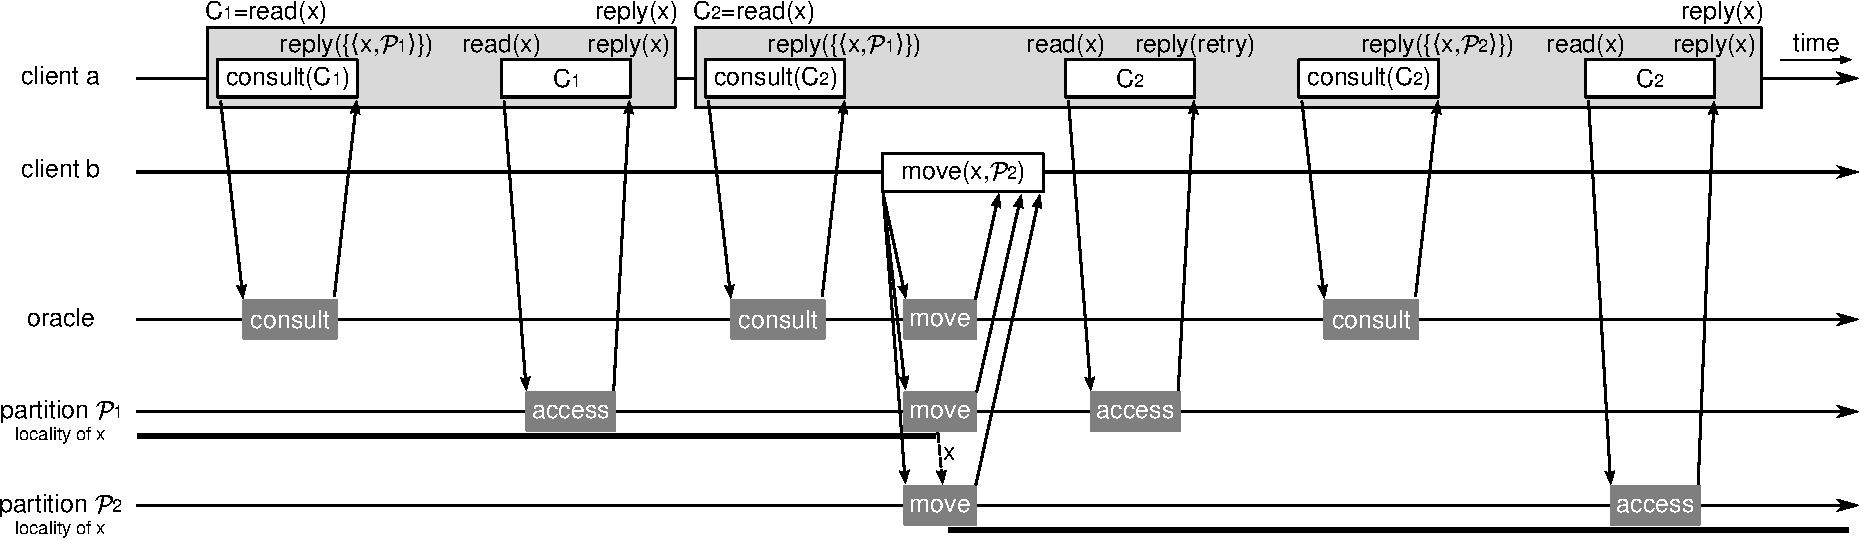
\includegraphics[width=1.0\linewidth]{figures/move_case_1}
%\end{minipage}
%\caption{Consulting the oracle and issuing a command are done in multiple calls to \amcast{}. White boxes represent actions of the client proxy.}
%\label{fig:move_case_1}
%\end{figure*}

%Algorithm~\ref{alg:ssmr} shows precisely how S-SMR operates. 
In more detail, when a server $s$ of partition $\ppm$, while executing a command $C$, needs to read variable $v$, there are two possibilities:
either $v$ belongs to the local partition $\ppm$,
or it is part of a remote partition $\ppm'$. 
If $v$ is local, $s$ will retrieve its value and send it to the servers of other partitions concerned by $C$;
if $v$ is remote, $s$ will wait until its value is received from a server of $\ppm'$. 
A write operation on $v$ does not depend on the previous value of $v$, not requiring communication between partitions, even if $v$ is not assigned to the partition of the server executing $C$.
To ensure linearizability, all partitions involved in the execution of a multi-partition command $C$ must coordinate before a reply can be sent to the client.
%To understand why, consider the non-linearizable execution shown in Figure~\ref{fig:whysignals}~(a).
%This execution is not linearizable because the only equivalent sequential execution requires $C_y$ to precede $C_{xy}$ and $C_{xy}$ to precede $C_x$, thus $C_y$ would precede $C_x$.
%Although this execution does not violate atomic order, it contradicts real-time ordering, in which $C_x$ precedes $C_y$.
In \ssmr{}, partitions exchange signals while executing multi-partition commands~\cite{bezerra2014ssmr}.
This guarantees linearizability, at the cost of synchronizing partitions.

S-SMR improves on classical SMR by allowing single-partition commands to scale. 
Multi-partition commands, however, have limited performance. 
One way to reduce the number of multi-partition commands is to dynamically put variables that are usually accessed together in the same partition.
Unfortunately, \ssmr 's static mapping of variables to partitions does not allow the service to dynamically adapt to different access patterns.

%\subsection{S-SMR with dynamic partitioning}
%\subsection{Scalable replication with decentralized dynamic state partitioning}
%\subsection{Dynamic decentralized state partitioning}
\subsection{Dynamic state partitioning (DS-SMR)}

\dssmr{}~\cite{hoang2016} defines a dynamic mapping of variables to partitions.
Each variable $v$ is mapped to a partition $\ppm$, that is, $v \in \ppm$.
Such a mapping is managed by the partitioning oracle, which, differently from \ssmr, is now implemented as a replicated service run by a group of server processes.
The oracle allows the mapping of variables to partitions to be retrieved or changed during execution.
In more detail, \dssmr\ distinguishes five types of commands:
$access(\omega)$ is an application command that accesses (reads or writes) variables in set $\omega \subseteq \vvm$,
$create(v)$ creates a new variable $v$ and initially maps it to a partition defined by the oracle,
$delete(v)$ removes $v$ from the service state,
% resulting in $part(v) = \emptyset$,
$move(v,\ppm_s,\ppm_d)$ moves variable $v$ from partition $\ppm_s$ to partition $\ppm_d$,
and $consult(C)$ asks the oracle which variables are accessed by command $C$, and which partition contains each of them.
The reply from the oracle is called a $prophecy$, and usually consists of a set of tuples $\langle v, \ppm \rangle$, meaning $v \in \ppm$.
% The other possible values for a prophecy are $ok$ and $nok$, which mean that command can and cannot be executed, respectively (more details in Section~\ref{sec:algorithm}).
%If $v$ is not part of the service state (i.e., it was deleted or never created), the prophecy will contain~$\langle v, \emptyset \rangle$.

% explain which partitions deliver each partitioning command:
% how are access, consult, create, move and delete implemented?

%Once the oracle is in place, 
Clients consult the oracle to know which partitions each command should be multicast to, based on the objects accessed by the command.
If the reply received from the oracle tells the client that the command accesses a single partition, the client multicasts the command to that partition.
If the command accesses objects from multiple partitions, the client first multicasts one or more $move$ commands to the oracle and to the involved partitions, with the intent of having all variables in the same partition.
Then, the command itself is multicast to the one partition that now holds all variables accessed by the command.
If a subsequent command accesses the same variables, it will also access a single partition.
Thus, the access patterns of commands will shape the mapping of variables to partitions, reducing the number of multi-partition commands.

Consulting the oracle and issuing the application command are done with separate calls to atomic multicast in \dssmr{}.
It may happen that, between those operations, the partitioning changes.
%We illustrate this in Figure~\ref{fig:move_case_1}.
%Commands $C_1$ and $C_2$ read variable $x$.
%Since partitioning is dynamic, the client issuing the commands first consults the oracle before multicasting each command.
%$C_1$ executes without the interference of other commands, so consulting the oracle and multicasting the command only once is enough for $C_1$ to be executed.
%However, before $C_2$ is multicast to $\ppm_1$, another client issues a $move$ command that relocates $x$ to $\ppm_2$.
%When $C_2$ is delivered at the servers of $\ppm_1$, the command is not executed, since $x$ is not available at $\ppm_1$ anymore.
%A similar situation may arise when a command accesses variables from multiple partitions, as it consists of multicasting at least three commands separately: $consult$, $move$ and $access$.
%The partitioning can change between the execution of any two of those commands.
%\begin{figure}[b!]
%  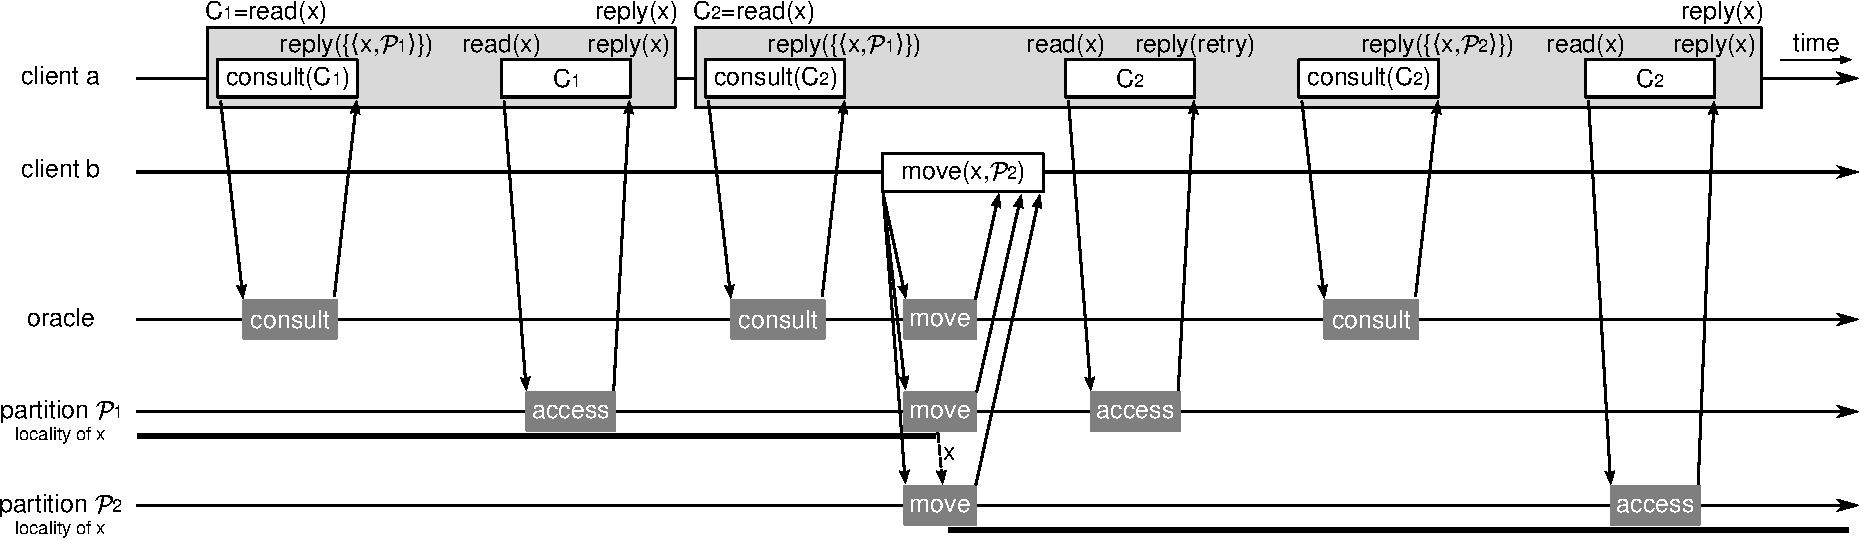
\includegraphics[width=\linewidth]{figures/move_case_1}
%  \caption{Consulting the oracle and issuing an application command consist of multiple calls to \amcast{}.}
%  \label{fig:move_case_1}
%\end{figure}
% \pagebreak
To solve this problem, the client multicasts the set of variables accessed along with each access command.
Upon delivery, each server checks the set of variables sent by the client.
If all variables in the set belong to the local partition, the command is executed; otherwise, a $retry$ message is sent back to the client.
When the client receives a $retry$ message, it consults the oracle again, possibly moves variables across partitions, and then reissues the access command.
To guarantee termination, if the command fails a certain number of times, the client multicasts the command to all partitions and the servers execute it as in the original \ssmr{}.

